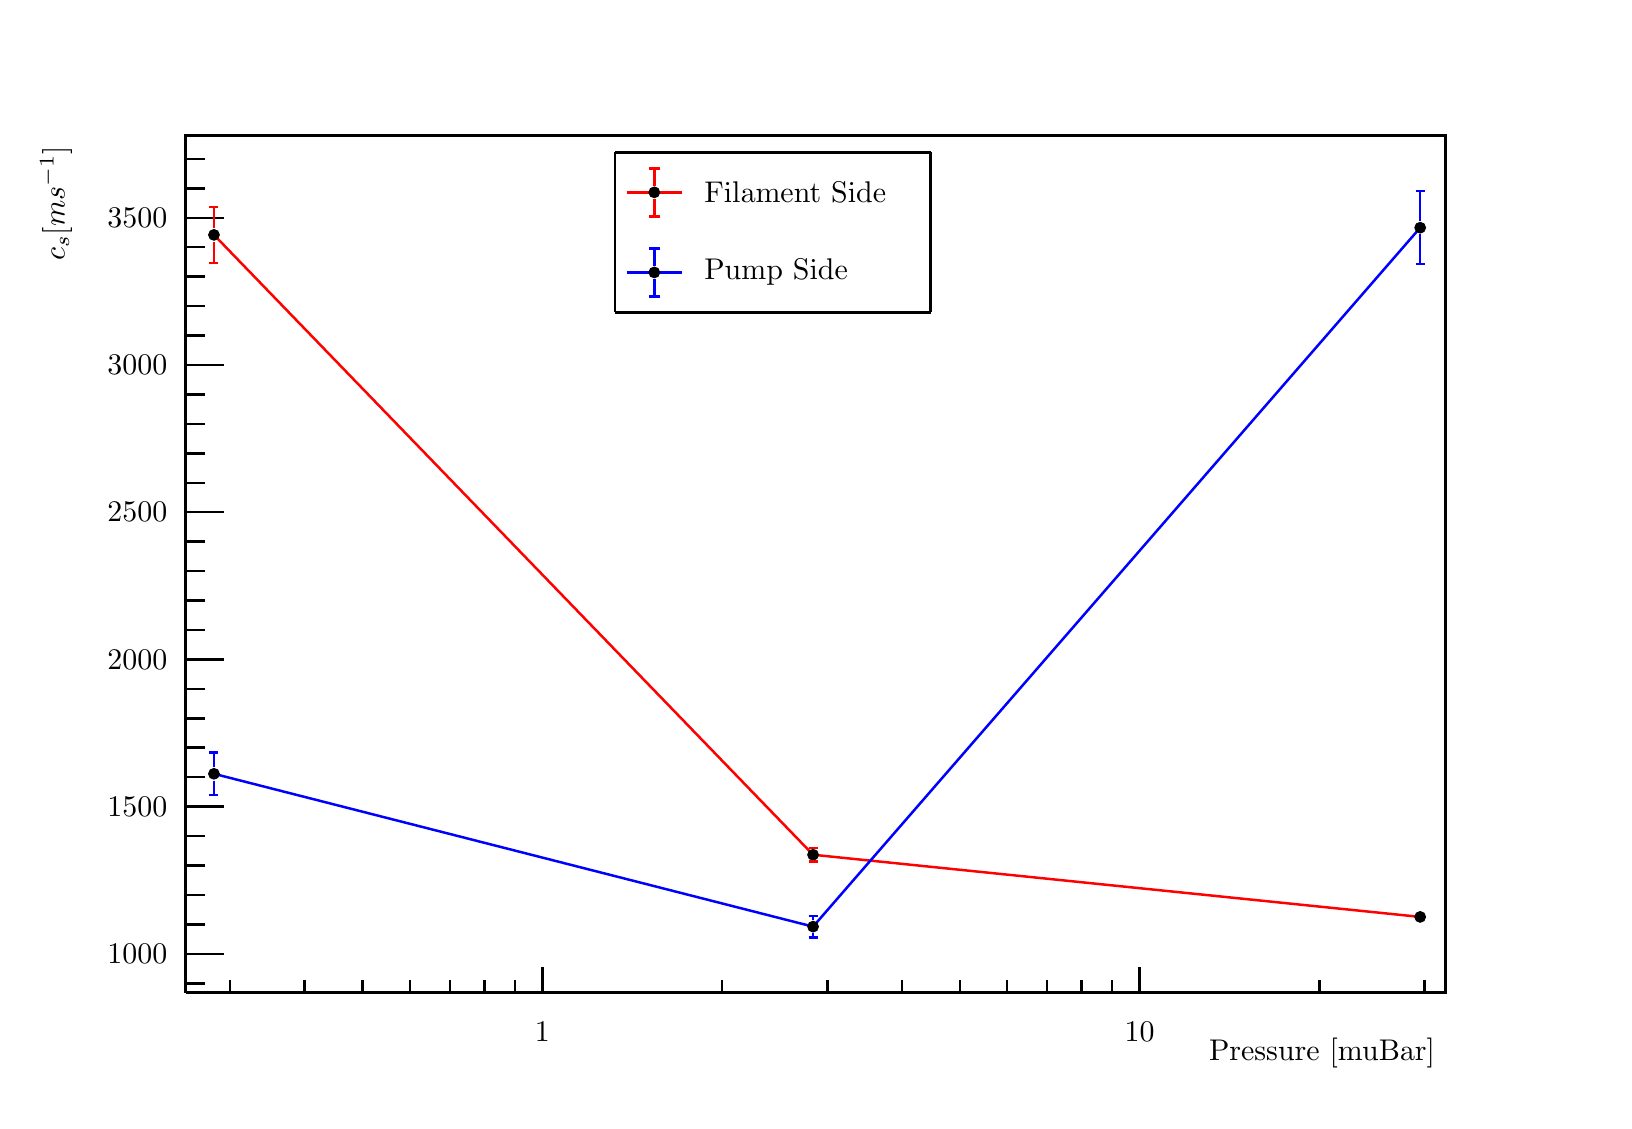
\begin{tikzpicture}
\pgfdeclareplotmark{cross} {
\pgfpathmoveto{\pgfpoint{-0.3\pgfplotmarksize}{\pgfplotmarksize}}
\pgfpathlineto{\pgfpoint{+0.3\pgfplotmarksize}{\pgfplotmarksize}}
\pgfpathlineto{\pgfpoint{+0.3\pgfplotmarksize}{0.3\pgfplotmarksize}}
\pgfpathlineto{\pgfpoint{+1\pgfplotmarksize}{0.3\pgfplotmarksize}}
\pgfpathlineto{\pgfpoint{+1\pgfplotmarksize}{-0.3\pgfplotmarksize}}
\pgfpathlineto{\pgfpoint{+0.3\pgfplotmarksize}{-0.3\pgfplotmarksize}}
\pgfpathlineto{\pgfpoint{+0.3\pgfplotmarksize}{-1.\pgfplotmarksize}}
\pgfpathlineto{\pgfpoint{-0.3\pgfplotmarksize}{-1.\pgfplotmarksize}}
\pgfpathlineto{\pgfpoint{-0.3\pgfplotmarksize}{-0.3\pgfplotmarksize}}
\pgfpathlineto{\pgfpoint{-1.\pgfplotmarksize}{-0.3\pgfplotmarksize}}
\pgfpathlineto{\pgfpoint{-1.\pgfplotmarksize}{0.3\pgfplotmarksize}}
\pgfpathlineto{\pgfpoint{-0.3\pgfplotmarksize}{0.3\pgfplotmarksize}}
\pgfpathclose
\pgfusepathqstroke
}
\pgfdeclareplotmark{cross*} {
\pgfpathmoveto{\pgfpoint{-0.3\pgfplotmarksize}{\pgfplotmarksize}}
\pgfpathlineto{\pgfpoint{+0.3\pgfplotmarksize}{\pgfplotmarksize}}
\pgfpathlineto{\pgfpoint{+0.3\pgfplotmarksize}{0.3\pgfplotmarksize}}
\pgfpathlineto{\pgfpoint{+1\pgfplotmarksize}{0.3\pgfplotmarksize}}
\pgfpathlineto{\pgfpoint{+1\pgfplotmarksize}{-0.3\pgfplotmarksize}}
\pgfpathlineto{\pgfpoint{+0.3\pgfplotmarksize}{-0.3\pgfplotmarksize}}
\pgfpathlineto{\pgfpoint{+0.3\pgfplotmarksize}{-1.\pgfplotmarksize}}
\pgfpathlineto{\pgfpoint{-0.3\pgfplotmarksize}{-1.\pgfplotmarksize}}
\pgfpathlineto{\pgfpoint{-0.3\pgfplotmarksize}{-0.3\pgfplotmarksize}}
\pgfpathlineto{\pgfpoint{-1.\pgfplotmarksize}{-0.3\pgfplotmarksize}}
\pgfpathlineto{\pgfpoint{-1.\pgfplotmarksize}{0.3\pgfplotmarksize}}
\pgfpathlineto{\pgfpoint{-0.3\pgfplotmarksize}{0.3\pgfplotmarksize}}
\pgfpathclose
\pgfusepathqfillstroke
}
\pgfdeclareplotmark{newstar} {
\pgfpathmoveto{\pgfqpoint{0pt}{\pgfplotmarksize}}
\pgfpathlineto{\pgfqpointpolar{44}{0.5\pgfplotmarksize}}
\pgfpathlineto{\pgfqpointpolar{18}{\pgfplotmarksize}}
\pgfpathlineto{\pgfqpointpolar{-20}{0.5\pgfplotmarksize}}
\pgfpathlineto{\pgfqpointpolar{-54}{\pgfplotmarksize}}
\pgfpathlineto{\pgfqpointpolar{-90}{0.5\pgfplotmarksize}}
\pgfpathlineto{\pgfqpointpolar{234}{\pgfplotmarksize}}
\pgfpathlineto{\pgfqpointpolar{198}{0.5\pgfplotmarksize}}
\pgfpathlineto{\pgfqpointpolar{162}{\pgfplotmarksize}}
\pgfpathlineto{\pgfqpointpolar{134}{0.5\pgfplotmarksize}}
\pgfpathclose
\pgfusepathqstroke
}
\pgfdeclareplotmark{newstar*} {
\pgfpathmoveto{\pgfqpoint{0pt}{\pgfplotmarksize}}
\pgfpathlineto{\pgfqpointpolar{44}{0.5\pgfplotmarksize}}
\pgfpathlineto{\pgfqpointpolar{18}{\pgfplotmarksize}}
\pgfpathlineto{\pgfqpointpolar{-20}{0.5\pgfplotmarksize}}
\pgfpathlineto{\pgfqpointpolar{-54}{\pgfplotmarksize}}
\pgfpathlineto{\pgfqpointpolar{-90}{0.5\pgfplotmarksize}}
\pgfpathlineto{\pgfqpointpolar{234}{\pgfplotmarksize}}
\pgfpathlineto{\pgfqpointpolar{198}{0.5\pgfplotmarksize}}
\pgfpathlineto{\pgfqpointpolar{162}{\pgfplotmarksize}}
\pgfpathlineto{\pgfqpointpolar{134}{0.5\pgfplotmarksize}}
\pgfpathclose
\pgfusepathqfillstroke
}
\definecolor{c}{rgb}{1,1,1};
\draw [color=c, fill=c] (0,0) rectangle (20,13.6103);
\draw [color=c, fill=c] (2,1.36103) rectangle (18,12.2493);
\definecolor{c}{rgb}{0,0,0};
\draw [c,line width=0.9] (2,1.36103) -- (2,12.2493) -- (18,12.2493) -- (18,1.36103) -- (2,1.36103);
\definecolor{c}{rgb}{1,1,1};
\draw [color=c, fill=c] (2,1.36103) rectangle (18,12.2493);
\definecolor{c}{rgb}{0,0,0};
\draw [c,line width=0.9] (2,1.36103) -- (2,12.2493) -- (18,12.2493) -- (18,1.36103) -- (2,1.36103);
\draw [c,line width=0.9] (2,1.36103) -- (18,1.36103);
\draw [c,line width=0.9] (2.56262,1.52436) -- (2.56262,1.36103);
\draw [c,line width=0.9] (3.51031,1.52436) -- (3.51031,1.36103);
\draw [c,line width=0.9] (4.2454,1.52436) -- (4.2454,1.36103);
\draw [c,line width=0.9] (4.84601,1.52436) -- (4.84601,1.36103);
\draw [c,line width=0.9] (5.35381,1.52436) -- (5.35381,1.36103);
\draw [c,line width=0.9] (5.79369,1.52436) -- (5.79369,1.36103);
\draw [c,line width=0.9] (6.1817,1.52436) -- (6.1817,1.36103);
\draw [c,line width=0.9] (6.52878,1.68768) -- (6.52878,1.36103);
\draw [anchor=base] (6.52878,0.745165) node[scale=1.08185, color=c, rotate=0]{1};
\draw [c,line width=0.9] (8.81216,1.52436) -- (8.81216,1.36103);
\draw [c,line width=0.9] (10.1479,1.52436) -- (10.1479,1.36103);
\draw [c,line width=0.9] (11.0955,1.52436) -- (11.0955,1.36103);
\draw [c,line width=0.9] (11.8306,1.52436) -- (11.8306,1.36103);
\draw [c,line width=0.9] (12.4312,1.52436) -- (12.4312,1.36103);
\draw [c,line width=0.9] (12.939,1.52436) -- (12.939,1.36103);
\draw [c,line width=0.9] (13.3789,1.52436) -- (13.3789,1.36103);
\draw [c,line width=0.9] (13.7669,1.52436) -- (13.7669,1.36103);
\draw [c,line width=0.9] (14.114,1.68768) -- (14.114,1.36103);
\draw [anchor=base] (14.114,0.745165) node[scale=1.08185, color=c, rotate=0]{10};
\draw [c,line width=0.9] (16.3974,1.52436) -- (16.3974,1.36103);
\draw [c,line width=0.9] (17.7331,1.52436) -- (17.7331,1.36103);
\draw [anchor= east] (18,0.598854) node[scale=1.08185, color=c, rotate=0]{Pressure [muBar]};
\draw [c,line width=0.9] (2,1.36103) -- (2,12.2493);
\draw [c,line width=0.9] (2.48,1.8552) -- (2,1.8552);
\draw [c,line width=0.9] (2.24,2.2291) -- (2,2.2291);
\draw [c,line width=0.9] (2.24,2.60299) -- (2,2.60299);
\draw [c,line width=0.9] (2.24,2.97689) -- (2,2.97689);
\draw [c,line width=0.9] (2.24,3.35079) -- (2,3.35079);
\draw [c,line width=0.9] (2.48,3.72469) -- (2,3.72469);
\draw [c,line width=0.9] (2.24,4.09858) -- (2,4.09858);
\draw [c,line width=0.9] (2.24,4.47248) -- (2,4.47248);
\draw [c,line width=0.9] (2.24,4.84638) -- (2,4.84638);
\draw [c,line width=0.9] (2.24,5.22028) -- (2,5.22028);
\draw [c,line width=0.9] (2.48,5.59417) -- (2,5.59417);
\draw [c,line width=0.9] (2.24,5.96807) -- (2,5.96807);
\draw [c,line width=0.9] (2.24,6.34197) -- (2,6.34197);
\draw [c,line width=0.9] (2.24,6.71587) -- (2,6.71587);
\draw [c,line width=0.9] (2.24,7.08976) -- (2,7.08976);
\draw [c,line width=0.9] (2.48,7.46366) -- (2,7.46366);
\draw [c,line width=0.9] (2.24,7.83756) -- (2,7.83756);
\draw [c,line width=0.9] (2.24,8.21145) -- (2,8.21145);
\draw [c,line width=0.9] (2.24,8.58535) -- (2,8.58535);
\draw [c,line width=0.9] (2.24,8.95925) -- (2,8.95925);
\draw [c,line width=0.9] (2.48,9.33315) -- (2,9.33315);
\draw [c,line width=0.9] (2.24,9.70704) -- (2,9.70704);
\draw [c,line width=0.9] (2.24,10.0809) -- (2,10.0809);
\draw [c,line width=0.9] (2.24,10.4548) -- (2,10.4548);
\draw [c,line width=0.9] (2.24,10.8287) -- (2,10.8287);
\draw [c,line width=0.9] (2.48,11.2026) -- (2,11.2026);
\draw [c,line width=0.9] (2.48,1.8552) -- (2,1.8552);
\draw [c,line width=0.9] (2.24,1.4813) -- (2,1.4813);
\draw [c,line width=0.9] (2.48,11.2026) -- (2,11.2026);
\draw [c,line width=0.9] (2.24,11.5765) -- (2,11.5765);
\draw [c,line width=0.9] (2.24,11.9504) -- (2,11.9504);
\draw [anchor= east] (1.9,1.8552) node[scale=1.08185, color=c, rotate=0]{1000};
\draw [anchor= east] (1.9,3.72469) node[scale=1.08185, color=c, rotate=0]{1500};
\draw [anchor= east] (1.9,5.59417) node[scale=1.08185, color=c, rotate=0]{2000};
\draw [anchor= east] (1.9,7.46366) node[scale=1.08185, color=c, rotate=0]{2500};
\draw [anchor= east] (1.9,9.33315) node[scale=1.08185, color=c, rotate=0]{3000};
\draw [anchor= east] (1.9,11.2026) node[scale=1.08185, color=c, rotate=0]{3500};
\draw [anchor= east] (0.354441,12.2493) node[scale=1.08185, color=c, rotate=90]{$c_s [m s^{-1}]$};
\definecolor{c}{rgb}{1,0,0};
\draw [c,line width=0.9] (2.35878,10.9858) -- (9.9673,3.11344) -- (17.6777,2.32399);
\definecolor{c}{rgb}{0,0,0};
\foreach \P in {(2.35878,10.9858), (9.9673,3.11344), (17.6777,2.32399)}{\draw[mark options={color=c,fill=c},mark size=1.921922pt,mark=*] plot coordinates {\P};}
\definecolor{c}{rgb}{1,0,0};
\draw [c,line width=0.9] (2.35878,11.0718) -- (2.35878,11.3419);
\draw [c,line width=0.9] (2.30148,11.3419) -- (2.41609,11.3419);
\draw [c,line width=0.9] (2.35878,10.8999) -- (2.35878,10.6298);
\draw [c,line width=0.9] (2.30148,10.6298) -- (2.41609,10.6298);
\draw [c,line width=0.9] (9.9673,3.1994) -- (9.9673,3.20035);
\draw [c,line width=0.9] (9.91,3.20035) -- (10.0246,3.20035);
\draw [c,line width=0.9] (9.9673,3.02748) -- (9.9673,3.02653);
\draw [c,line width=0.9] (9.91,3.02653) -- (10.0246,3.02653);
\definecolor{c}{rgb}{0,0,1};
\draw [c,line width=0.9] (2.35878,4.2275) -- (2.35878,4.41219);
\draw [c,line width=0.9] (2.30148,4.41219) -- (2.41609,4.41219);
\draw [c,line width=0.9] (2.35878,4.05558) -- (2.35878,3.8709);
\draw [c,line width=0.9] (2.30148,3.8709) -- (2.41609,3.8709);
\draw [c,line width=0.9] (9.9673,2.28642) -- (9.9673,2.33598);
\draw [c,line width=0.9] (9.91,2.33598) -- (10.0246,2.33598);
\draw [c,line width=0.9] (9.9673,2.1145) -- (9.9673,2.06493);
\draw [c,line width=0.9] (9.91,2.06493) -- (10.0246,2.06493);
\draw [c,line width=0.9] (17.6777,11.163) -- (17.6777,11.5399);
\draw [c,line width=0.9] (17.6204,11.5399) -- (17.735,11.5399);
\draw [c,line width=0.9] (17.6777,10.991) -- (17.6777,10.6141);
\draw [c,line width=0.9] (17.6204,10.6141) -- (17.735,10.6141);
\draw [c,line width=0.9] (2.35878,4.14154) -- (9.9673,2.20046) -- (17.6777,11.077);
\definecolor{c}{rgb}{0,0,0};
\foreach \P in {(2.35878,4.14154), (9.9673,2.20046), (17.6777,11.077)}{\draw[mark options={color=c,fill=c},mark size=1.921922pt,mark=*] plot coordinates {\P};}
\definecolor{c}{rgb}{1,1,1};
\draw [color=c, fill=c] (7.44986,10) rectangle (11.4613,12.0344);
\definecolor{c}{rgb}{0,0,0};
\draw [c,line width=0.9] (7.44986,10) -- (11.4613,10);
\draw [c,line width=0.9] (11.4613,10) -- (11.4613,12.0344);
\draw [c,line width=0.9] (11.4613,12.0344) -- (7.44986,12.0344);
\draw [c,line width=0.9] (7.44986,12.0344) -- (7.44986,10);
\draw [anchor= west] (8.45272,11.5258) node[scale=1.08185, color=c, rotate=0]{Filament Side};
\definecolor{c}{rgb}{1,0,0};
\draw [c,line width=0.9] (7.60029,11.5258) -- (8.30229,11.5258);
\draw [c,line width=0.9] (7.95129,11.6117) -- (7.95129,11.8309);
\draw [c,line width=0.9] (7.95129,11.4398) -- (7.95129,11.2206);
\draw [c,line width=0.9] (7.88109,11.8309) -- (8.02149,11.8309);
\draw [c,line width=0.9] (7.88109,11.2206) -- (8.02149,11.2206);
\definecolor{c}{rgb}{0,0,0};
\foreach \P in {(7.95129,11.5258)}{\draw[mark options={color=c,fill=c},mark size=1.921922pt,mark=*] plot coordinates {\P};}
\draw [anchor= west] (8.45272,10.5086) node[scale=1.08185, color=c, rotate=0]{Pump Side};
\definecolor{c}{rgb}{0,0,1};
\draw [c,line width=0.9] (7.60029,10.5086) -- (8.30229,10.5086);
\draw [c,line width=0.9] (7.95129,10.5946) -- (7.95129,10.8138);
\draw [c,line width=0.9] (7.95129,10.4226) -- (7.95129,10.2034);
\draw [c,line width=0.9] (7.88109,10.8138) -- (8.02149,10.8138);
\draw [c,line width=0.9] (7.88109,10.2034) -- (8.02149,10.2034);
\definecolor{c}{rgb}{0,0,0};
\foreach \P in {(7.95129,10.5086)}{\draw[mark options={color=c,fill=c},mark size=1.921922pt,mark=*] plot coordinates {\P};}
\end{tikzpicture}
